% Originally: content/week-09.tex, \subsection{Volume of embedded surfaces} --- promoted to a section

\section{Volume of embedded surfaces}
\label{sec:volume_embedded_surfaces}

% Source: Corsin Nick/Class Notes/Week 9.pdf, p. 5
% Def. 13.68
\begin{definition}[$d$-volume on a parametrized $d$-submanifold]
\label{def:d_volume_parametrized_submanifold}
Let $V \subseteq \mathbb{R}^d$ be open, and let $\phi : V \to \mathbb{R}^n$ be a parametrized
submanifold. Given a Jordan measurable set $E \subseteq V$ with $\overline E \subseteq V$,
we define the $d$-volume of $\phi(E)$ by
\[\vol_d(\phi(E)) := \int_E \sqrt{\det\big(D\phi(x)\transp D\phi(x)\big)}\,dx.\]
\end{definition}

Here the Gram determinant in the integrand is the volume of the parallelotope spanned by the
vectors $\partial_1\phi(x),\partial_2\phi(x),\dots,\partial_d\phi(x)$, which by assumption
(see \qt{parametrized submanifold}) are linearly independent --- i.e.\ $D\phi(x)$ has full
rank --- so the volume is strictly positive.

% Sonnet 5 (Medium) --- FIG-W09-03
\begin{center}
\begin{tikzpicture}[>=Latex, scale=1.3]
  \draw[thick] plot[smooth] coordinates {(-2.1,-0.4) (-0.8,0.65) (0.5,-0.15) (2.1,0.75)};
  \draw[thick] plot[smooth] coordinates {(-1.8,0.9) (-0.5,-0.5) (0.8,0.4) (2.3,-0.65)};
  \coordinate (P) at (0.0,0.05);
  \fill (P) circle (1.6pt) node[below left, font=\scriptsize] {$\phi(x)$};
  \draw[blue, thick, ->] (P) -- ++(1.2,0.4) coordinate (D1)
    node[right, font=\scriptsize] {$\partial_1\phi(x)$};
  \draw[purple, thick, ->] (P) -- ++(0.35,1.05) coordinate (D2)
    node[above, font=\scriptsize] {$\partial_2\phi(x)$};
  \draw[green!55!black, dashed]
    (D1) -- ++(0.35,1.05) -- (D2) -- cycle;
  \node[green!45!black, font=\scriptsize, align=center] at (2.1,1.5)
    {$\sqrt{D\phi(x)\transp D\phi(x)}$};
  \draw[green!55!black, thin, ->] (1.55,1.3) -- (0.95,1.0);
\end{tikzpicture}
\end{center}

This factor gives a measure for the stretching of $E$ as it is \qt{glued} to the surface. If
\[\sqrt{D\phi(x)\transp D\phi(x)} = 1 \quad \text{for all } x,\]
then $\phi$ is called an \newterm{isometry} (\germanterm{Isometrie}). A special case is the
length of a curve, treated in \cref{sec:length_of_curve} below.

% Supplement: Sascha Brack/Class Notes/Week_09_Notes_Friday.pdf, p. 3
\begin{example}[Integral on the graph of a function]
\label{ex:integral_graph_function}
Given an open set $U \subseteq \mathbb{R}^2$ and a $C^1$ function $f: U \to \mathbb{R}$, we can define the parametrized surface $\phi: U \to \mathbb{R}^3$ by $\phi(x,y) = (x,y,f(x,y))\transp$.
Assuming $M := \operatorname{Im}\phi$ is a $C^1$ submanifold, its area is given by $\int_M 1 \mathop{d\text{vol}}_2$.

We first find the Jacobian matrix of the parametrization:
\[\Jac\phi(x,y) = \begin{pmatrix} 1 & 0 \\ 0 & 1 \\ \partial_1 f(x,y) & \partial_2 f(x,y) \end{pmatrix}.\]
Then we compute the Gram determinant:
\begin{align*}
\sqrt{|\det(\Jac\phi\transp \Jac\phi)|}
&= \sqrt{\det \begin{pmatrix} 1+(\partial_1 f)^2 & \partial_1 f \partial_2 f \\ \partial_2 f \partial_1 f & 1+(\partial_2 f)^2 \end{pmatrix}} \\
&= \sqrt{\big(1+(\partial_1 f)^2\big)\big(1+(\partial_2 f)^2\big) - (\partial_1 f)^2(\partial_2 f)^2} \\
&= \sqrt{1 + (\partial_1 f)^2 + (\partial_2 f)^2} = \sqrt{1+|\nabla f(x,y)|^2}.
\end{align*}
By definition, we get the surface area formula for a graph:
\[\int_M 1 \mathop{d\text{vol}}_2 = \int_U \sqrt{1+|\nabla f(x,y)|^2} \,dx\,dy.\]
\end{example}

\subsection{Example: area of a paraboloid patch}
\label{sec:example_paraboloid_area}

% Source: Corsin Nick/Class Notes/Week 9.pdf, pp. 6--7
\begin{example}[Area of a paraboloid patch]
\label{ex:paraboloid_patch_area}
Compute the area of the surface
\[F = \left\{(x,y,z)\in\mathbb{R}^3 \ :\ x^2+4y^2 < 8,\ \ z = \tfrac12(x^2+2y^2)\right\}.\]

Since $z = \tfrac12(x^2+2y^2)$ means $F$ is a graph, we can conveniently write $F$ as the
image of the parametrization
\[\phi : A \to F, \qquad (x,y) \mapsto \left(x,\,y,\,\tfrac12(x^2+2y^2)\right),
  \qquad A := \{(x,y)\in\mathbb{R}^2 : x^2+4y^2 < 8\}.\]

\textbf{Gram determinant.} We compute
\[D\phi(x,y) = \begin{pmatrix} 1 & 0 \\ 0 & 1 \\ x & 2y \end{pmatrix}
  \quad \Longrightarrow \quad
  D\phi(x,y)\transp D\phi(x,y) = \begin{pmatrix} 1+x^2 & 2xy \\ 2xy & 1+4y^2 \end{pmatrix},\]
so that
\[\sqrt{\det D\phi(x,y)\transp D\phi(x,y)}
  = \sqrt{(1+x^2)(1+4y^2) - 4x^2y^2}
  = \sqrt{1+x^2+4y^2}.\]

\textbf{The integral.} By \cref{def:d_volume_parametrized_submanifold},
\[\vol_2(F) = \int_A \sqrt{1+x^2+4y^2}\,dx\,dy, \qquad A = \{(x,y)\in\mathbb{R}^2 :
x^2+4y^2<8\}.\]

We should choose more convenient coordinates. Polar coordinates come to mind, but then we
still have problems, since $A$ is not radially symmetric. We want to write
$A = \Psi\big((0,R)\times(0,2\pi)\big)$ (up to a set of measure zero). Note that for $y=0$,
$|x| < \sqrt8 = 2\sqrt2$, and for $x=0$, $|y| < \sqrt2$. Choosing $R := \sqrt2$ and weighing
$x,y$ accordingly,
\[\begin{pmatrix} x \\ y \end{pmatrix} = \begin{pmatrix} 2r\cos\theta \\ r\sin\theta
\end{pmatrix} =: \Psi(r,\theta).\]

\textbf{Change of variables.}
\[dx\,dy = |\det D\Psi(r,\theta)|\,dr\,d\theta
  = \left\lVert \begin{matrix} 2\cos\theta & -2r\sin\theta \\ \sin\theta & r\cos\theta
    \end{matrix}\right\rVert dr\,d\theta = 2r\,dr\,d\theta,\]
giving
\[
\begin{aligned}
\vol_2(F) &= \int_A \sqrt{1+x^2+4y^2}\,dx\,dy
  = \int_0^{\sqrt2} dr\int_0^{2\pi} d\theta\ 2r\sqrt{1+4r^2} \\
  &= 4\pi\int_0^{\sqrt2} dr\ r(1+4r^2)^{1/2}
   = \frac\pi2\int_0^{\sqrt2} dr\ 8r(1+4r^2)^{1/2} \\
  &= \frac\pi2\left[(1+4r^2)^{3/2}\cdot\frac23\right]_0^{\sqrt2}
   = \frac\pi3\big(27-1\big) = \frac{26\pi}{3}.
\end{aligned}
\]
\end{example}

\begin{ainote}
Worth flagging what makes $A$ awkward: it is an ellipse, not a disc, so naive polar
coordinates $(x,y)=(\rho\cos\theta,\rho\sin\theta)$ would force $\rho$ to depend on $\theta$
along the boundary. The fix is to build the eccentricity into the change of variables itself
--- scaling $x$ by a factor of $2$ relative to $y$ turns the ellipse into the disc $r<\sqrt2$
before polar coordinates are even applied. This is the same idea as
\Cref{ex:change_of_variables_domain}: choose $\Psi$ to straighten the domain, not
to simplify the integrand.
\end{ainote}

% Supplement: Sascha Brack/Class Notes/Week_09_Notes_Monday.pdf, p. 7
\begin{example}[Surface area of a sphere]
\label{ex:surface_area_sphere}
Given the sphere $M := \{(x,y,z) \in \mathbb{R}^3 \mid x^2+y^2+z^2 = r^2\}$, we can use the parametrization $\phi : (0,\pi) \times (-\pi,\pi) \to \mathbb{R}^3$,
\[\phi(\theta,\varphi) = \begin{pmatrix} r\sin\theta\cos\varphi \\ r\sin\theta\sin\varphi \\ r\cos\theta \end{pmatrix}.\]
The Jacobian matrix is
\[\Jac\phi(\theta,\varphi) = \begin{pmatrix} r\cos\theta\cos\varphi & -r\sin\theta\sin\varphi \\ r\cos\theta\sin\varphi & r\sin\theta\cos\varphi \\ -r\sin\theta & 0 \end{pmatrix},\]
which has rank 2 for all $(\theta,\varphi)$ in the domain.
Then we compute the Gram determinant:
\[\Jac\phi\transp \Jac\phi = \begin{pmatrix} r^2 & 0 \\ 0 & r^2\sin^2\theta \end{pmatrix} \quad \Longrightarrow \quad \sqrt{\det(\Jac\phi\transp \Jac\phi)} = r^2\sin\theta.\]
The surface area is given by the integral:
\begin{align*}
\int_M 1 \mathop{d\text{vol}}_2 &= \int_{-\pi}^\pi \int_0^\pi \sqrt{\det(\Jac\phi\transp \Jac\phi)} \,d\theta\,d\varphi \\
&= \int_{-\pi}^\pi \int_0^\pi r^2\sin\theta \,d\theta\,d\varphi \\
&= r^2 \left(\int_{-\pi}^\pi d\varphi\right) \left(\int_0^\pi \sin\theta \,d\theta\right) \\
&= r^2 \cdot 2\pi \cdot 2 = 4\pi r^2.
\end{align*}
Note that here, our partition of unity simply was the identity (since the parametrization covers the sphere up to a null set).

\begin{center}
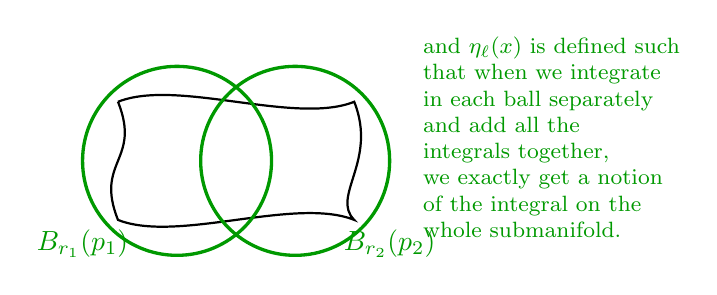
\begin{tikzpicture}[scale=1.5]
  % Submanifold shape
  \draw[thick] (0,0) .. controls (0.5,0.2) and (1.5,-0.2) .. (2,0)
               .. controls (2.2,-0.5) and (1.8,-0.8) .. (2,-1)
               .. controls (1.5,-0.8) and (0.5,-1.2) .. (0,-1)
               .. controls (-0.2,-0.5) and (0.2,-0.5) .. (0,0);
               
  % Two charts
  \draw[very thick, green!60!black] (0.5,-0.5) circle (0.8);
  \node[green!60!black] at (-0.3,-1.2) {$B_{r_1}(p_1)$};
  
  \draw[very thick, green!60!black] (1.5,-0.5) circle (0.8);
  \node[green!60!black] at (2.3,-1.2) {$B_{r_2}(p_2)$};
  
  \node[right, font=\footnotesize, align=left, text=green!60!black] at (2.5, -0.3) {
    and $\eta_\ell(x)$ is defined such\\
    that when we integrate\\
    in each ball separately\\
    and add all the\\
    integrals together,\\
    we exactly get a notion\\
    of the integral on the\\
    whole submanifold.
  };
\end{tikzpicture}
\end{center}
\end{example}


% --- exercises relocated here from the dissolved sheet 9 ---

% Originally: content/week-09.tex, \exercisesheet{9}, problem 9.1
% Source: exercises/Ex9_Analysis2_eng.pdf

% Source: exercises/Ex9_Analysis2_eng.pdf, p. 1
\begin{exercise}[9.1 --- Volume \textnormal{(important)}]
\label{ex:9.1}
Calculate the volume of the region $B \subset \mathbb{R}^3$ enclosed by the surfaces
$x^2+y^2+z^2=8$ and $2z=x^2+y^2$. \textit{Official hint:} use cylindrical coordinates.

% Source: Corsin Nick/Class Notes/Week 9.pdf, p. 1
\textit{Corsin's hint:}
\[\begin{pmatrix} x \\ y \\ z\end{pmatrix} = \begin{pmatrix} r\sin\theta\cos\varphi \\
  r\sin\theta\sin\varphi \\ r\cos\theta \end{pmatrix}
  \qquad \text{for } (r,\theta,\varphi) \in (0,\infty)\times(0,\pi)\times(0,2\pi).\]
\end{exercise}

\begin{ainote}
Corsin labels the formula above \qt{cylindrical coordinates}, but $(r\sin\theta\cos\varphi$, $r\sin\theta\sin\varphi$, $r\cos\theta)$ is the \textbf{spherical} parametrization, and his
range $\theta \in (-\pi/2,\pi/2)$ has been corrected to $(0,\pi)$, the range on which
$\theta \mapsto \cos\theta$ actually covers $[-1,1]$ bijectively (already logged in \cref{ex:7.6}). The mislabelling is doubly worth noting here, since the official sheet's own hint
recommends \emph{cylindrical} coordinates $(r,\theta,z)$ --- and that is in fact the more
natural choice for this problem, as \cref{ex:solution_9.1} below uses: both surfaces are
surfaces of revolution about the $z$-axis, which cylindrical coordinates respect directly,
whereas spherical coordinates mix $r$ and $\theta$ into both defining equations.
\end{ainote}
